% Options for packages loaded elsewhere
\PassOptionsToPackage{unicode}{hyperref}
\PassOptionsToPackage{hyphens}{url}
%
\documentclass[
]{book}
\usepackage{lmodern}
\usepackage{amssymb,amsmath}
\usepackage{ifxetex,ifluatex}
\ifnum 0\ifxetex 1\fi\ifluatex 1\fi=0 % if pdftex
  \usepackage[T1]{fontenc}
  \usepackage[utf8]{inputenc}
  \usepackage{textcomp} % provide euro and other symbols
\else % if luatex or xetex
  \usepackage{unicode-math}
  \defaultfontfeatures{Scale=MatchLowercase}
  \defaultfontfeatures[\rmfamily]{Ligatures=TeX,Scale=1}
\fi
% Use upquote if available, for straight quotes in verbatim environments
\IfFileExists{upquote.sty}{\usepackage{upquote}}{}
\IfFileExists{microtype.sty}{% use microtype if available
  \usepackage[]{microtype}
  \UseMicrotypeSet[protrusion]{basicmath} % disable protrusion for tt fonts
}{}
\makeatletter
\@ifundefined{KOMAClassName}{% if non-KOMA class
  \IfFileExists{parskip.sty}{%
    \usepackage{parskip}
  }{% else
    \setlength{\parindent}{0pt}
    \setlength{\parskip}{6pt plus 2pt minus 1pt}}
}{% if KOMA class
  \KOMAoptions{parskip=half}}
\makeatother
\usepackage{xcolor}
\IfFileExists{xurl.sty}{\usepackage{xurl}}{} % add URL line breaks if available
\IfFileExists{bookmark.sty}{\usepackage{bookmark}}{\usepackage{hyperref}}
\hypersetup{
  pdftitle={Indicadores de gestión por procesos},
  pdfauthor={ Oficina Nacional de Estadística   Sistema Integrado de Gestión - SIGA},
  hidelinks,
  pdfcreator={LaTeX via pandoc}}
\urlstyle{same} % disable monospaced font for URLs
\usepackage{longtable,booktabs}
% Correct order of tables after \paragraph or \subparagraph
\usepackage{etoolbox}
\makeatletter
\patchcmd\longtable{\par}{\if@noskipsec\mbox{}\fi\par}{}{}
\makeatother
% Allow footnotes in longtable head/foot
\IfFileExists{footnotehyper.sty}{\usepackage{footnotehyper}}{\usepackage{footnote}}
\makesavenoteenv{longtable}
\usepackage{graphicx}
\makeatletter
\def\maxwidth{\ifdim\Gin@nat@width>\linewidth\linewidth\else\Gin@nat@width\fi}
\def\maxheight{\ifdim\Gin@nat@height>\textheight\textheight\else\Gin@nat@height\fi}
\makeatother
% Scale images if necessary, so that they will not overflow the page
% margins by default, and it is still possible to overwrite the defaults
% using explicit options in \includegraphics[width, height, ...]{}
\setkeys{Gin}{width=\maxwidth,height=\maxheight,keepaspectratio}
% Set default figure placement to htbp
\makeatletter
\def\fps@figure{htbp}
\makeatother
\setlength{\emergencystretch}{3em} % prevent overfull lines
\providecommand{\tightlist}{%
  \setlength{\itemsep}{0pt}\setlength{\parskip}{0pt}}
\setcounter{secnumdepth}{5}
\usepackage{booktabs}
\usepackage[]{natbib}
\bibliographystyle{apalike}

\title{Indicadores de gestión por procesos}
\usepackage{etoolbox}
\makeatletter
\providecommand{\subtitle}[1]{% add subtitle to \maketitle
  \apptocmd{\@title}{\par {\large #1 \par}}{}{}
}
\makeatother
\subtitle{Guía Metodológica}
\author{ Oficina Nacional de Estadística Sistema Integrado de Gestión - SIGA}
\date{Versión 1.0}

\begin{document}
\maketitle

{
\setcounter{tocdepth}{1}
\tableofcontents
}
\hypertarget{portada}{%
\chapter*{Portada}\label{portada}}
\addcontentsline{toc}{chapter}{Portada}

\begin{center}
\includegraphics[width=0.75\linewidth]{Imagenes/Portada} \end{center}

Esta guía ha sido publicada por la Universidad Nacional de Colombia. La versión en línea de este documento está disponible bajo la licencia Creative Commons Attribution-NonCommercial-NoDerivatives 4.0 International.

\hypertarget{intro}{%
\chapter*{Introducción}\label{intro}}
\addcontentsline{toc}{chapter}{Introducción}

El Capítulo \ref{procesos}, titulado \emph{Gestión por procesos}, presenta el Sistema de \ldots{}

\hypertarget{procesos}{%
\chapter{Gestión por procesos}\label{procesos}}

El \emph{mapa de macroprocesos de la Universidad}, como se ilustra en la Figura \ref{fig:fig2}, está conformado por 16 macroprocesos.

\begin{figure}

{\centering 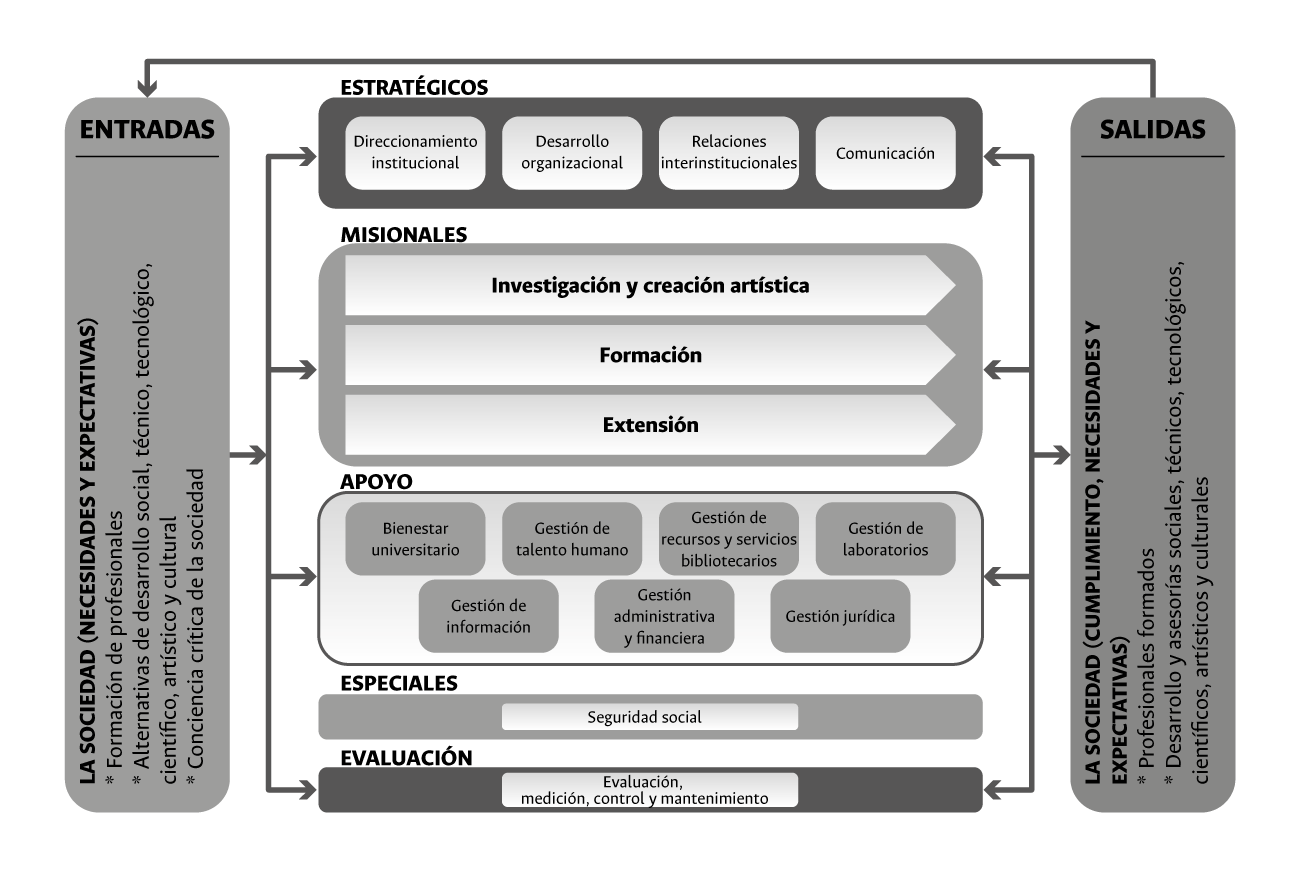
\includegraphics[width=0.8\linewidth]{Imagenes/F_2} 

}

\caption{Mapa de procesos institucionales. Tomado de Gestión por procesos en http://siga.unal.edu.co/index.php/procesos/gestion-por-procesos1.}\label{fig:fig2}
\end{figure}

\hypertarget{medicion}{%
\chapter{Seguimiento y medición}\label{medicion}}

Seguimiento, medición, análisis y evaluación

\hypertarget{alcance}{%
\section{Alcance}\label{alcance}}

\hypertarget{medidas}{%
\chapter{Tipos de medidas}\label{medidas}}

Existen tres tipos de medidas

\hypertarget{estaduxedsticas}{%
\section{Estadísticas}\label{estaduxedsticas}}

Como lo presenta \citet{Alberto2019}, las estadísticas\footnote{Nombre que se emplea para diferenciarlo de \ldots{}}

\hypertarget{indicadores-estaduxedsticos}{%
\section{Indicadores estadísticos}\label{indicadores-estaduxedsticos}}

\hypertarget{indicadores-de-cumplimiento}{%
\section{Indicadores de cumplimiento}\label{indicadores-de-cumplimiento}}

\hypertarget{indicadoresUN}{%
\chapter{Medición de los procesos en la UN}\label{indicadoresUN}}

\hypertarget{principios}{%
\section{Principios}\label{principios}}

\hypertarget{gobernabilidad}{%
\section{Gobernabilidad}\label{gobernabilidad}}

\hypertarget{un-proceso-especial}{%
\section{Un proceso especial}\label{un-proceso-especial}}

\hypertarget{anexos}{%
\chapter*{Anexos}\label{anexos}}
\addcontentsline{toc}{chapter}{Anexos}

  \bibliography{book.bib,packages.bib}

\end{document}
